\paragraph{Observation composition at fixed dimension.}
To separate coordinate composition from input dimension, all three paired subsets $\mathcal O_{ij}=\{x_i,x_j,e_i,e_j\}$, with $ij\in\{12,13,23\}$, are evaluated at each of Nodes 2 and 3. This completes the two-actuator-location by three-paired-subset comparison, not all arbitrary four-coordinate subsets. Each configuration has three independently trained policies with a nominal budget of $4\times10^5$ transitions. Six additional policies complete the previously missing Node 2/$\mathcal O_{13}$ and Node 3/$\mathcal O_{12}$ configurations. All six configurations are evaluated on 20 new common initial conditions, with unchanged dynamics, reward, action bounds, and PPO settings. Every final checkpoint is retained. This evaluation set differs from that in the preceding dimension-reduction comparison.

\begin{table}[pos=htbp,width=\linewidth]
\centering
\caption{Complete paired four-dimensional observation comparison at Nodes 2 and 3. Entries are mean $\pm$ sample standard deviation across three training-run means over 20 common initial conditions.}
\label{tab:observation_identity}
\small
\begin{tabular}{cccc}
\toprule
Node & Subset & MAE & $E_u$\\
\midrule
2 & $\mathcal O_{12}$ & $0.9104\pm0.1312$ & $9.60\pm3.59$\\
2 & $\mathcal O_{13}$ & $0.6253\pm0.0032$ & $150.68\pm38.64$\\
2 & $\mathcal O_{23}$ & $0.0866\pm0.0059$ & $9.64\pm0.81$\\
3 & $\mathcal O_{12}$ & $0.5235\pm0.0115$ & $209.02\pm25.40$\\
3 & $\mathcal O_{13}$ & $0.0438\pm0.0009$ & $6.85\pm0.39$\\
3 & $\mathcal O_{23}$ & $0.0771\pm0.0175$ & $142.70\pm154.59$\\
\bottomrule
\end{tabular}
\end{table}

\begin{figure*}[pos=!t,width=\textwidth]
\centering
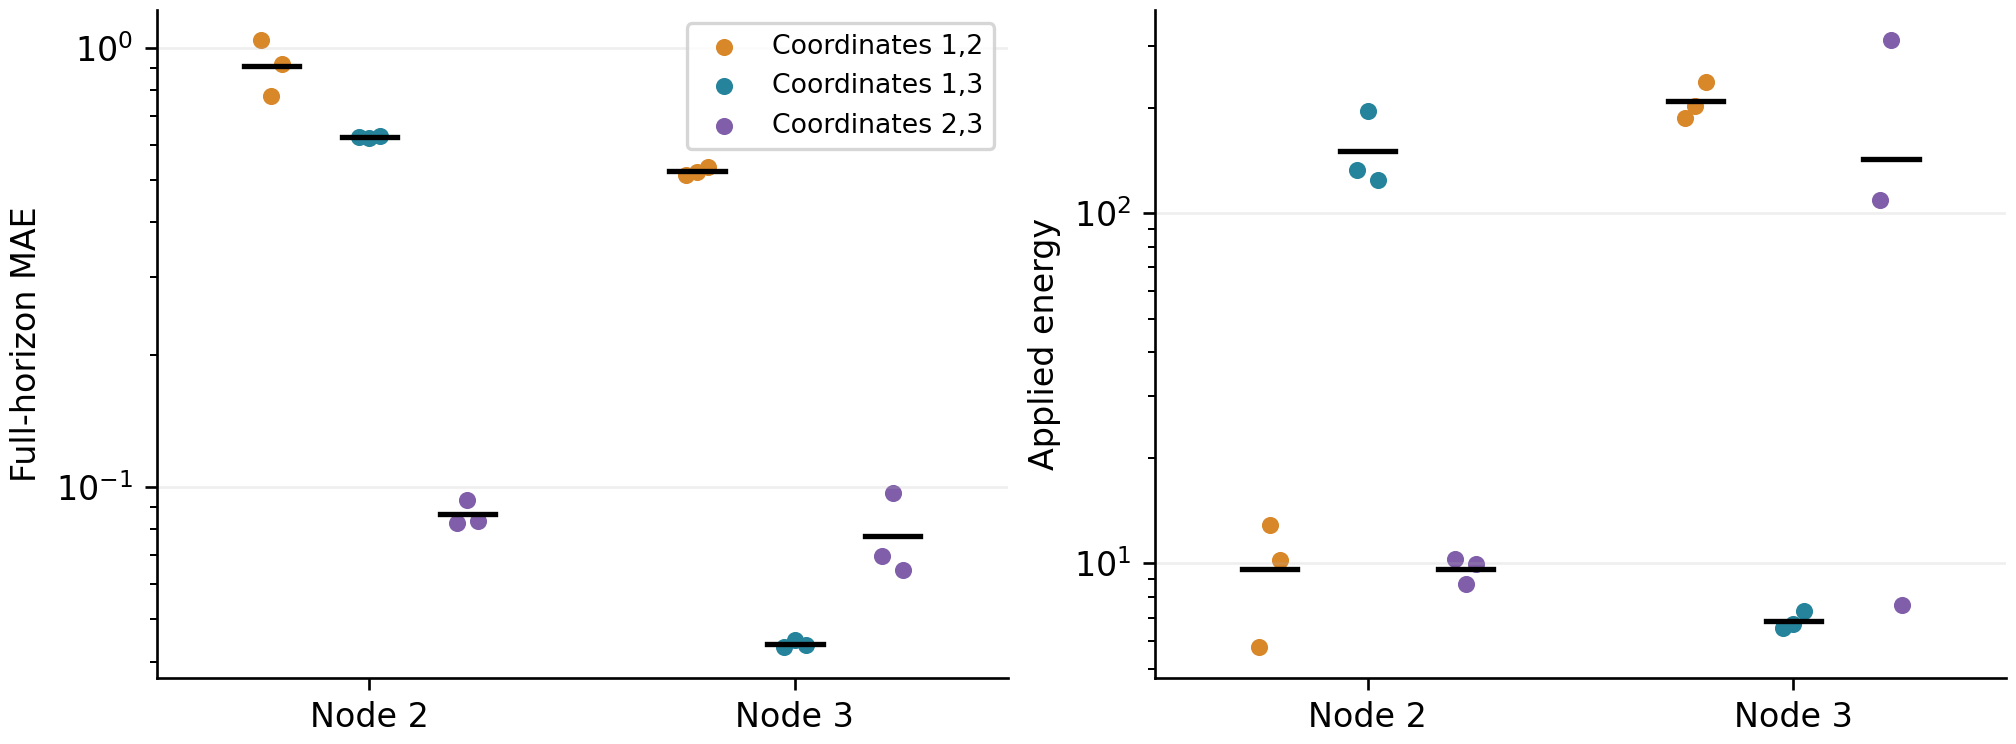
\includegraphics[width=0.92\textwidth]{figures/paired_observation_complete.png}
\caption{All paired four-dimensional subsets under single-node actuation. Each coordinate pair includes its drive states and error components. Points are individual training-run means over 20 common initial conditions; black marks average the three runs. Both error and energy are shown on logarithmic scales.}
\label{fig:observation_identity}
\end{figure*}

Table~\ref{tab:observation_identity} and Fig.~\ref{fig:observation_identity} confirm the actuator-dependent effect of coordinate composition. Node 2 performs best among these paired subsets with $\mathcal O_{23}$, whereas Node 3 favors $\mathcal O_{13}$ in both mean MAE and energy. The subsets omitting the actuated node's state--error pair, namely Node 2/$\mathcal O_{13}$ and Node 3/$\mathcal O_{12}$, give much larger residuals and energy than these favorable configurations. However, including that pair is not sufficient for low residuals: Node 2/$\mathcal O_{12}$ remains poor. Thus, the identity of the accompanying coordinate also matters. These are finite-budget learning results, not a proof that local information is necessary or that a particular subset is intrinsically optimal. At Node 3, $\mathcal O_{23}$ also exhibits substantial energy variability across training runs; none is excluded.
